\subsection{Quản lý video recap}

Người dùng có thể quản lý video recap của mình thông qua chức năng này. Hệ thống cho phép người dùng xem và theo dõi tiến độ tạo video của mình theo thời gian thực như Hình \ref{fig:video_recap}.

\begin{figure}[H]
    \centering
    \begin{subfigure}{0.32\textwidth}
        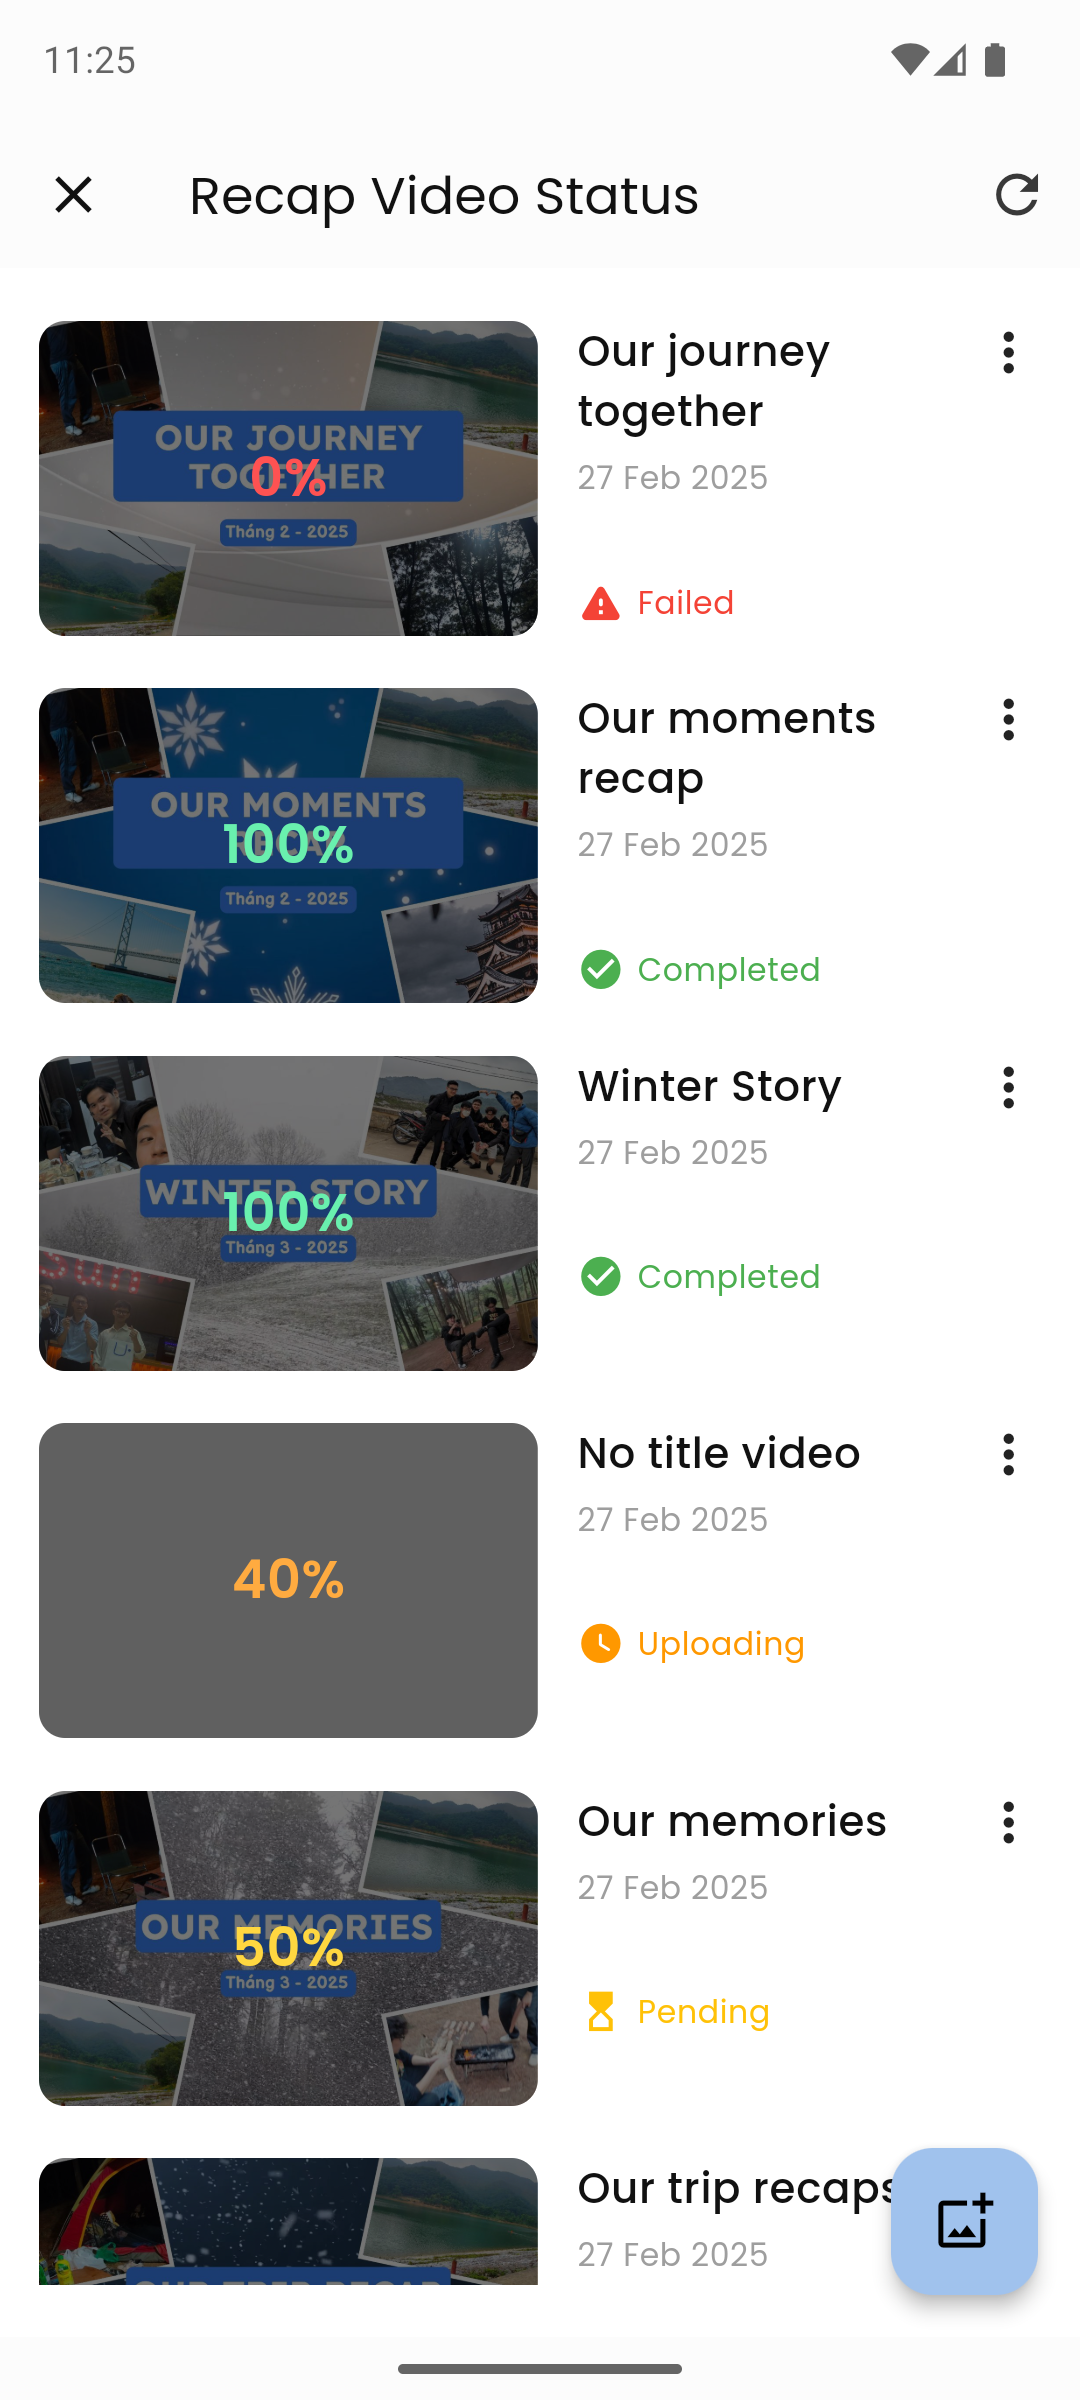
\includegraphics[width=1\linewidth]{figures/c4/4-2/video_1.png} 
        \caption{Danh sách video}
    \end{subfigure}
    \hfill
    \begin{subfigure}{0.32\textwidth}
        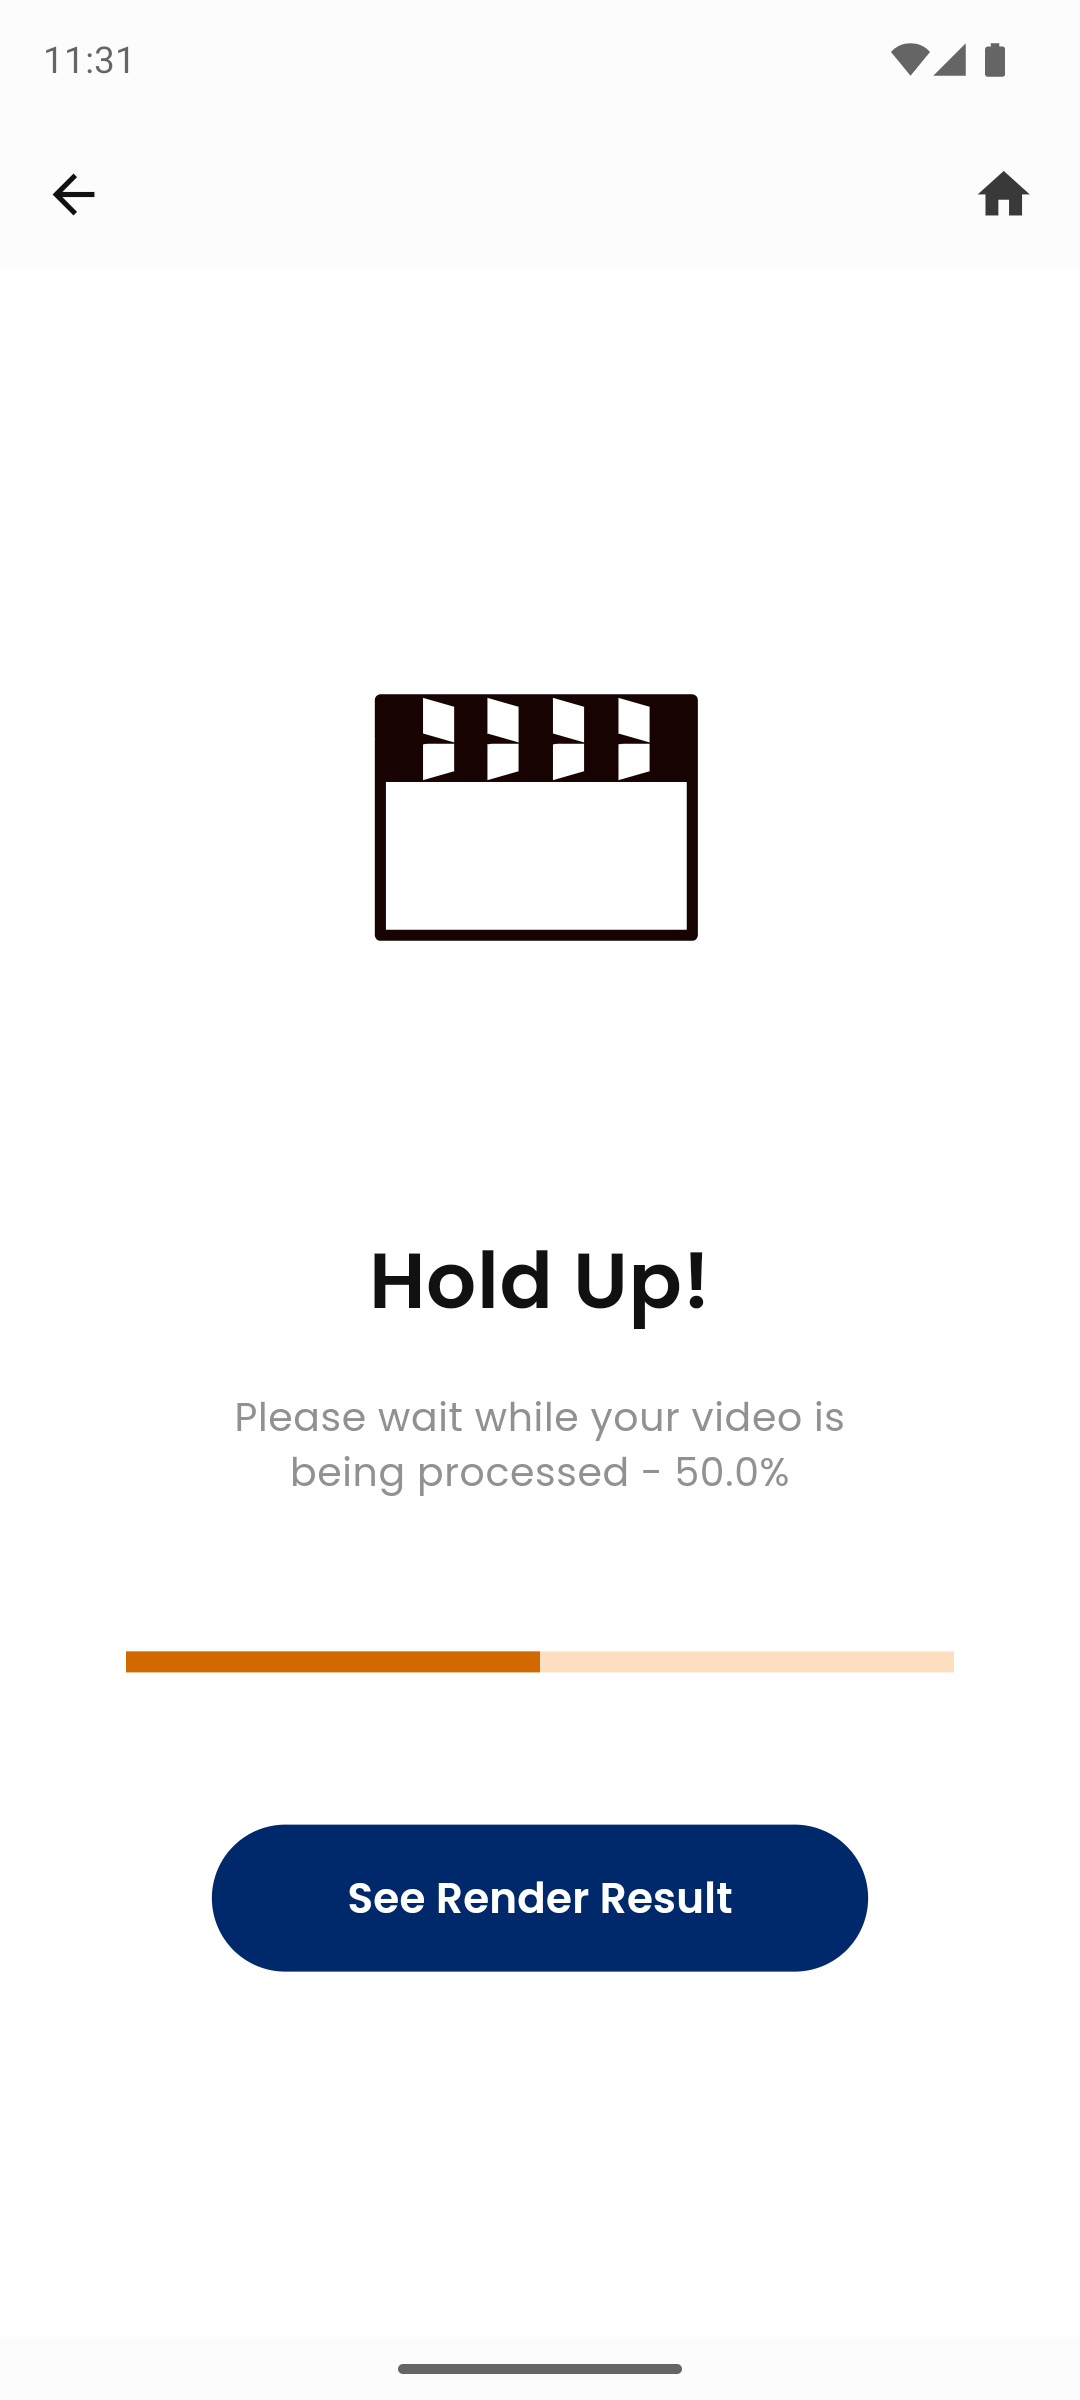
\includegraphics[width=1\linewidth]{figures/c4/4-2/video_2.png} 
        \caption{Xem trạng thái tạo video}
    \end{subfigure}
    \hfill
    \begin{subfigure}{0.32\textwidth}
        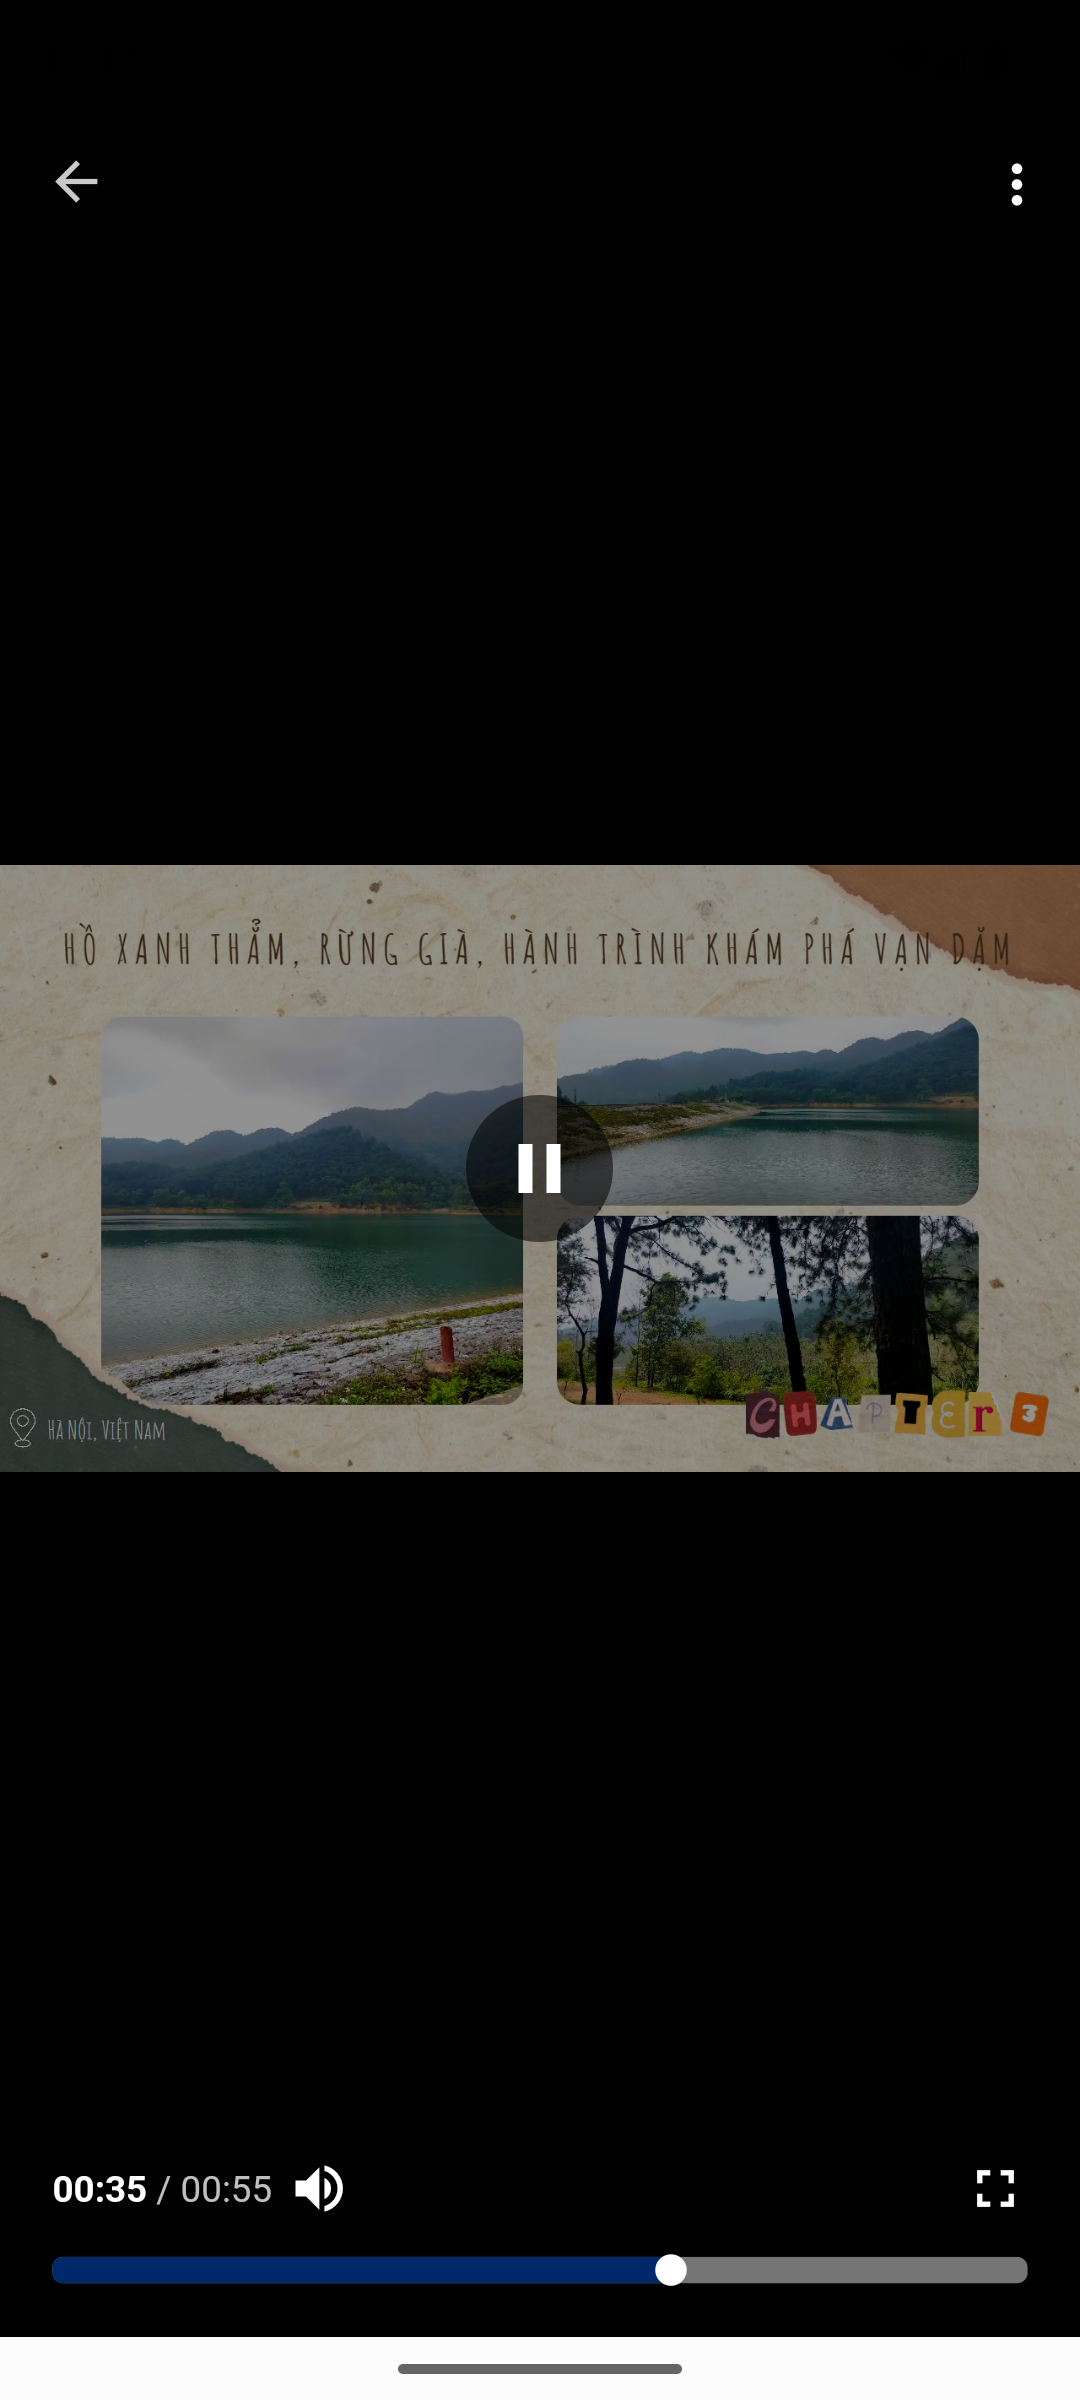
\includegraphics[width=1\linewidth]{figures/c4/4-2/video_3.png} 
        \caption{Xem video}
    \end{subfigure}
    \caption{Giao diện quản lý video recap.}
    \label{fig:video_recap}
\end{figure}

Ngoài ra, hệ thống cũng cung cấp tính năng tạo video cho người dùng và tùy chỉnh nhiều tùy chọn của video như chất lượng, chủ đề, nhạc nền, tiêu đề, v.v. như Hình \ref{fig:video_create}.

\begin{figure}[H]
    \centering
    \begin{subfigure}{0.48\textwidth}
        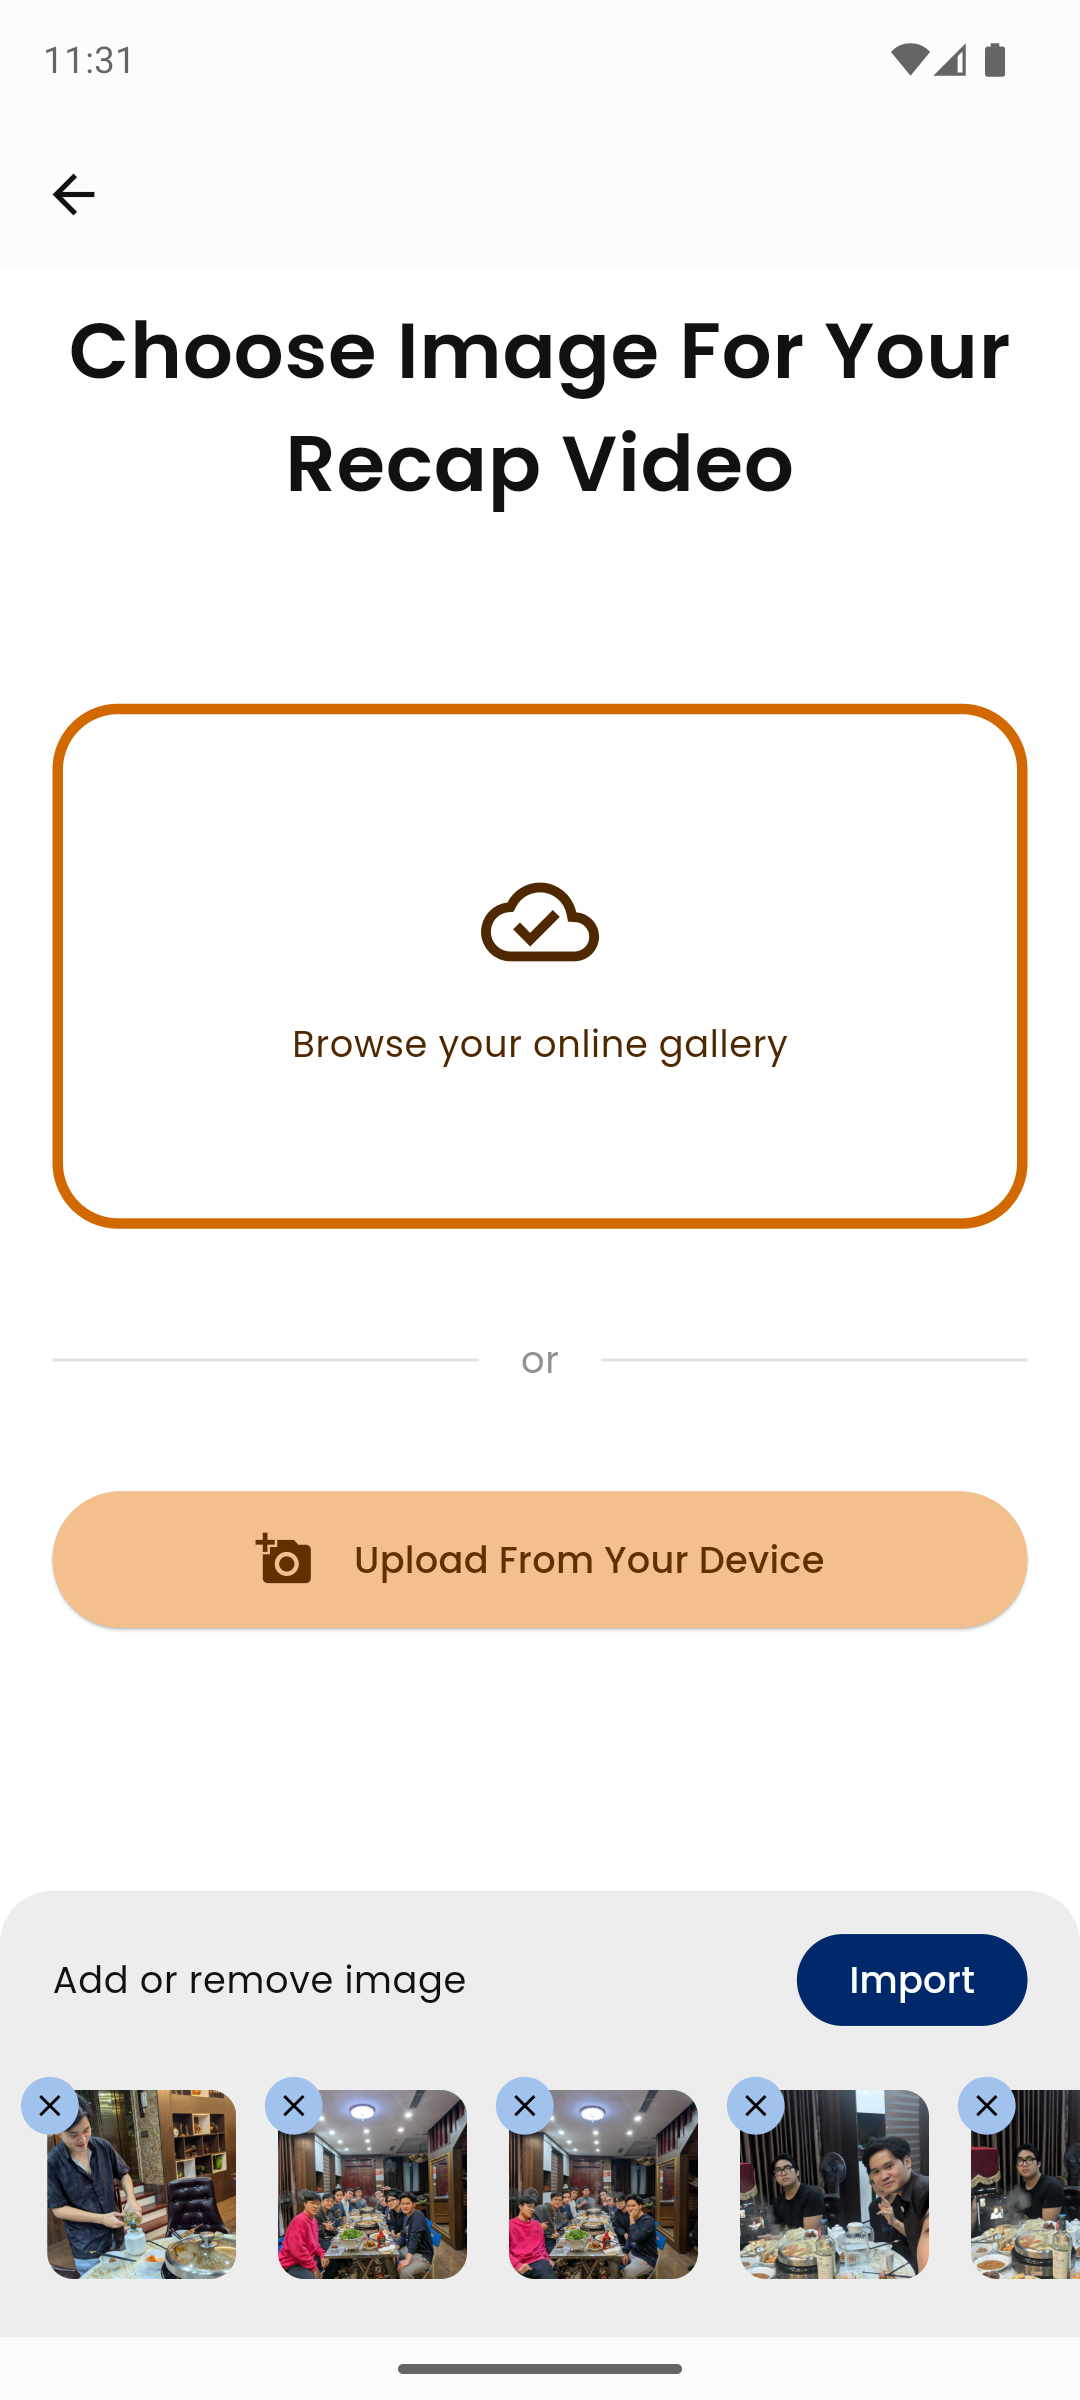
\includegraphics[width=1\linewidth]{figures/c4/4-2/create_video_1.png} 
        \caption{Tạo video}
    \end{subfigure}
    \hfill
    \begin{subfigure}{0.48\textwidth}
        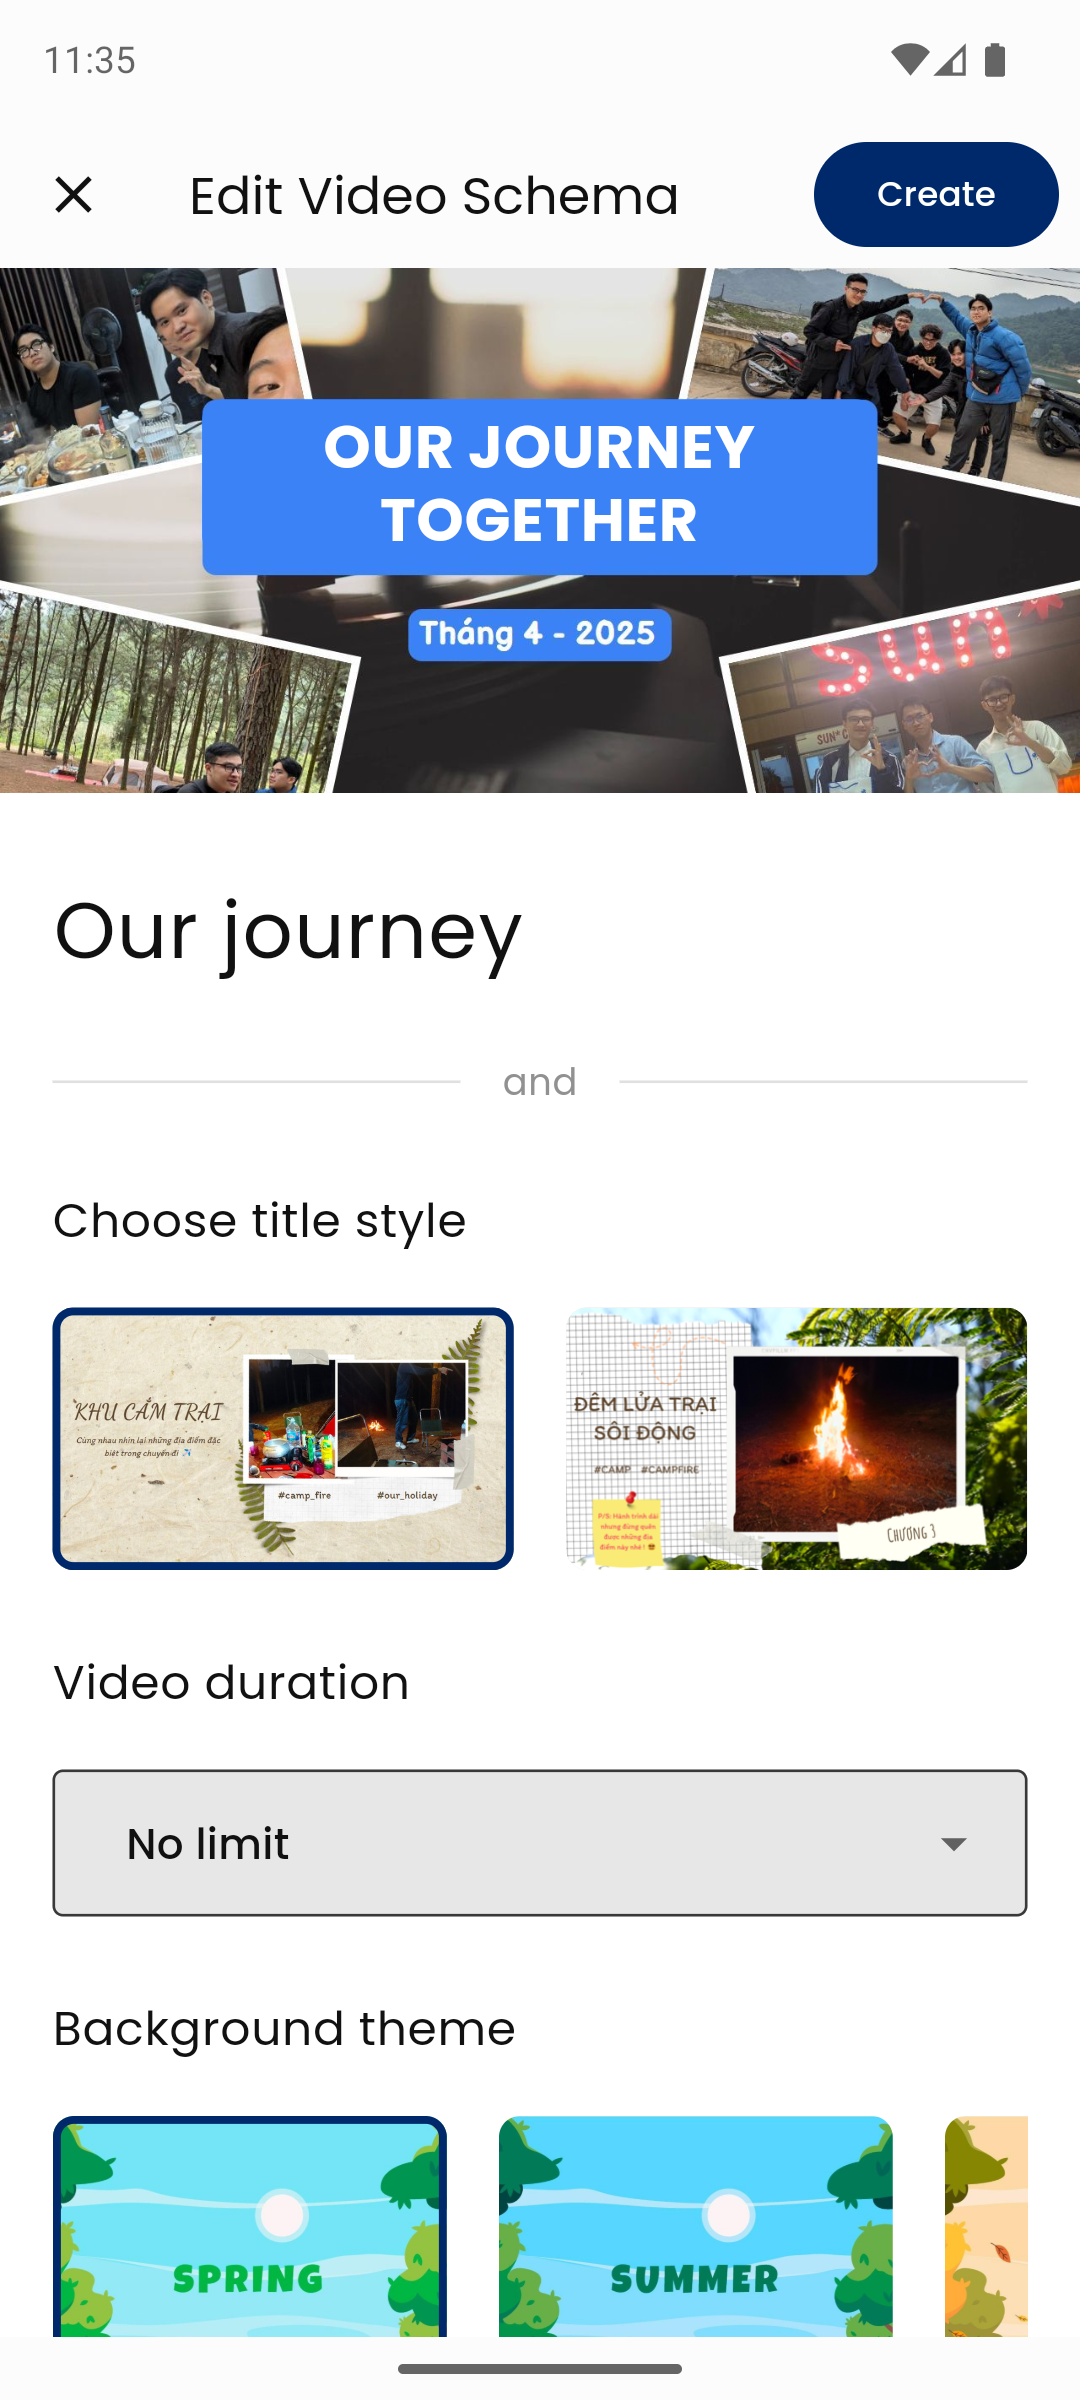
\includegraphics[width=1\linewidth]{figures/c4/4-2/create_video_2.png} 
        \caption{Chỉnh sửa tùy chọn video}
    \end{subfigure}
    \caption{Giao diện tạo video.}
    \label{fig:video_create}
\end{figure}